% Template"Advanced control techniques" project

\documentclass[a4paper,11pt,oneside]{book}
\usepackage[latin1]{inputenc}
\usepackage[english]{babel}
\usepackage{amsfonts}
\usepackage{amsmath}
\usepackage{amssymb,amsmath,color,psfrag}
\usepackage[draft]{graphicx}
\usepackage{cite}
\usepackage{url}
\usepackage{hyperref}
\usepackage{algorithm}
\usepackage{algorithmicx}
\usepackage{algpseudocode}
\usepackage{tabularx}
\usepackage{comment}
\usepackage{listings}
\usepackage[svgnames]{xcolor}
\usepackage{subcaption}

\lstset{ 
    backgroundcolor=\color{white},   
    basicstyle=\scriptsize\rmfamily,        
    breaklines=true,                 
    captionpos=b,           
    numbers=left,
    numberstyle=\tiny\color{Gray},         
    commentstyle=\color{Green},  
    escapeinside={\%*}{*)},          
    keywordstyle=\color{Blue},       
    stringstyle=\color{Black},  
    frameround=ftff,
    language=python,  
    frame=single,
    belowcaptionskip=3em,
    belowskip=2em,
}

\begin{document}
\pagestyle{myheadings}

\thispagestyle{empty}                                                 
\begin{center}                                                            
    \vspace{5mm}                                                           
 {\LARGE UNIVERSIT\`A DEL SALENTO} \\                       
      \vspace{5mm}
\end{center}
\begin{center}
{
\includegraphics[scale=.20]{figs/logo_unisalento}}      
\end{center}
\begin{center}
      \vspace{5mm}
      {\LARGE Facolt\`a di Ingegneria} \\
        \vspace{3mm}
      {\Large Corso di Laurea Magistrale in Computer Engineering} \\
      \vspace{20mm}
      {\LARGE Advanced Control Techniques Project} \\
      \vspace{5mm}{\LARGE\textbf{Multinomial Logistic Regression}}                  
      \vspace{15mm}
\end{center}
\begin{flushleft}                                                                              
     {\large Professor: \textbf{\@ Giuseppe Notarstefano}} \\        
      \vspace{13mm}
\end{flushleft}
\begin{flushright}
      {\large Students: \textbf{\@ Alfarano Gianluca,\\ Basile Davide,\\ Capoccia Leonardo,\\ Larini Ludovico}}\\
\end{flushright}        %capoverso allineato a destra
\begin{center}
\vfill
      {\large Academic year \@ 2017/2018} \\
\end{center}


\newpage
\thispagestyle{empty}

%%%%%% ABSTRACT %%%%%%%%%%
\begin{center}
\chapter*{}
\thispagestyle{empty}
{\Huge \textbf{Abstract}}\\
\vspace{15mm}
\end{center}
In this report, it will be shown how to solve a \textit{Multinomial Logistic Regression} problem (also known as \textit{Softmax Regression}) using a distributed approach. The \textit{Sub-gradient Method} has been used to distribute calculations among a configurable number of agents. A portion of the dataset is given to each agent and used to minimize a cost function related to the portion of the dataset in its possession.
The script solving the problem has been written using \textit{Python 3}. The most important library used is \textit{MPI4py} which provides implementation of the \textit{MPI} environment. \textit{MPI} is a communication protocol between nodes that executes the same program in parallel \cite{CITATION:4}. The results found with the distributed approach have been compared with the results obtained through a \textit{MATLAB} script, which executes all the operation using a centralized architecture (meaning that all operations are executed by a single agent).\\

%%%%%%%%%%%%%%%%%%%%%%%%%%%

\tableofcontents \thispagestyle{empty}
\listoffigures\thispagestyle{empty}

%%%%%% INTRODUZIONE %%%%%%%%%%
\chapter*{Introduction}
\addcontentsline{toc}{chapter}{Introduction}

\section*{Motivations}
In the past there was a single \textit{Mainframe} that executed all digital computations. Years after, with the creation of the \textit{Personal Computer}, more people could execute the same operations in private. Today's \textit{Micro controllers} allow to make smart all kind of devices. More algorithms have been created to connect these devices to distribute computations and tasks.\\
 In general, this approach is useful because it allows cooperation between agents and permits to reach a common goal. In this case, the ability to split the workload into several agents guarantees faster execution times.\\
The \textit{Multinomial Logistic Regression} for a multi-class classification problem, will be solved using a distributed approach in a faster way with respect to the same solution using a centralized method.

\section*{Contributions}
This work implements a scenario in which there are some agents that estimate a cost function using their own information and those of other agents; they use a \textit{Distributed Sub-gradient Method} to update their own estimates and, in particular, they solve a \textit{Multinomial Logistic Regression} problem.\\

The first step was to create a \textit{MATLAB} script that solves a quadratic optimization problem using a gradient method. In this script it has been \textit{simulated} a distributed approach in order to test the effectiveness of the method saw in \textit{Distributed Sub-gradient Methods} for Multi-Agent Optimization \cite{CITATION:1}. \textit{MATLAB} was only used in the prototype phase, because it doesn't allow real parallel computations. After the confirmation that the approach was working, the implementation of the algorithm in \textit{Python 3} using the \textit{Message Passing Interface} was started.\\
The quadratic form used was 
\begin{equation} \tag{I}
\dfrac{1}{2}x^{\top}Qx + r^{\top}x
\end{equation}
using
\begin{equation} \tag{II}
	Qx + r
\end{equation}
as gradient. This form was used only to test the convergence of the method and it was used as base to build the distributed script on it.\\
After having proved the convergence, considering that the \textit{Supervised Learning} problem known as \textit{Multinomial Logistic Regression} gives as output a probability value for every considered class, it was necessary to implement the \textit{Softmax function}. 
\begin{equation} \tag{III}
g_i\left(\theta\right):=\sum_{k=1}^{K}{1\{y^{(i)}=e_k\}\log{\left( \frac{exp(\theta^{(k)^\top}x^{(i)})}{\sum_{k=1}^{K}{exp( \theta^{(j)^\top}x )}} \right)}}
\end{equation} \\
\cite{CITATION:3}. This formula, which will be explained in Chapter \ref{Subsec1.1.2}, has been minimized in a centralized set-up using a \textit{MATLAB} script, and the result has been compared to the one of the \textit{Python} distributed script.\\
At the end, several tests has been executed to find the optimal values for the step-size.\\

% \section*{Organization}
%%%%%%%%%%%%%%%%%%%%%%%%%%%%%%%


%%%%%%%%%%%%%%%%%%%%%%%%%%%%%%%%%%%%
%%%%%%%%% CAPITOLO  %%%%%%%%%%%%%%%%
%%%%%%%%%%%%%%%%%%%%%%%%%%%%%%%%%%%%
\chapter{Problem and its implementation} \label{Cap1}

\section{Theory of the problem} \label{Sec1.1}
\subsection {Distributed Subgradient Methods for Multi-Agent Optimization} \label{Subsec1.1.1}
In this problem there are $m$ agents that cooperatively minimize a common additive cost. The general optimization problem is:\\
\begin{equation} \label{costfunct}
min \quad \sum\limits_{i=1}^{m} f_{i} \left( x \right) \qquad subject \ to \quad x \in \mathbb{R}^n,
\end{equation}
where $f_i : \mathbb{R}^n \longrightarrow \mathbb{R}$ is the cost function of agent $i$, known only by the agent $i$, and $x \in \mathbb{R}^n$ is the decision variable. It is assumed that:
\begin{itemize} 
\item the cost functions are convex;
\item the agents are distributed over a time-varying topology;
\item the graph $\left(V,E_\infty\right)$ is connected, where $E_\infty$ is the set of edges $\left(j,i\right)$ representing agent pairs communicating directly an indefinite number of times;
\item there is no communication delay.
\end{itemize} 
Each agent $i$ generates and maintains an estimate of the optimal decision variable based on the gradient of its own cost function and the exchanged estimates of its neighbours at discrete times $t_0, t_1, t_2, ...$. A weights matrix $A$ is associated to the communication graph, and its elements are defined as follows:
\[
	\begin{cases}
		a^i_i(k) \ge \eta & \text{for each } k \\
		a^i_j(k) \ge \eta, & \text{if } (j,i) \in E(k) \\
		a^i_j(k) = 0, & \text{otherwise}
	\end{cases}
\]
with $\eta$ defined as a strictly positive constant.\\
Each agent $i$ that receives an information by a neighbouring agent $j$ weights this information by multiplying it by $a_j^i(k) \in \mathbb{R}$. Then the estimate of the optimal solution is updated according to:
\begin{equation} \label{update}
x^i\left(k+1\right) = \sum_{j=1}^{m}{a_j^i\left(k\right)x^i\left(k\right)-\alpha^i\left(k\right)d_i\left(k\right)}
\end{equation}
where $\alpha^i(k)>0$ is the step-size used by agent $i$ and the vector $d_i(k)$ is a sub-gradient of the objective function $f_i(x)$ calculated at $x=x^i(k)$. \cite{CITATION:1}

\subsection {Multinomial Logistic Regression} \label{Subsec1.1.2}
The problem to be solved is a Supervised Learning problem called Multinomial Logistic Regression, also known as Softmax Regression. It generalizes the more common Logistic Regression. The difference between them is that in the former there are several classes to be considered, in the latter, there are only two classes (or equivalently a binary class).\\
The problem to be solved is to find a set of coefficients based on a given dataset to predict the belonging class for an unseen set of features, while minimizing a cost function. The dataset is composed of \textit{N} labelled examples $\{(x^{(1)}, y^{(1)}), ..., (x^{(N)}, y^{(N)})\}$. Each $x^{(i)} \in R^{d_{x}}$ for $i=1, ..., N$ is composed of some features which represent the value upon which is based the estimation of the belonging class, while $y^{(i)} \in \{ 1, \dots, K \}$ is the belonging class for the \textit{i-th} example.

Given a single training example $(x^{(i)}, y^{(i)})$, the definition of the cost function is:
\begin{equation}
f_i\left(\omega\right):=\left|\left|h_\omega\left(x^{(i)}\right)-y^{(i)}\right|\right|^2
\end{equation}
where the $\omega \in R^{d_{x}}$ are the weights of the hypothesis function $h_{\omega}$. The overall cost function can be defined as:
\begin{equation}
f\left(\omega\right):=\sum_{i=1}^{N}{f_i\left(\omega\right)}
\end{equation}
The problem is solved by finding the solution of the following optimization problem:
\begin{equation}
\omega^*:=\arg\min_\omega f\left(\omega\right)
\end{equation}
In the Multinomial Logistic Regression, a common choice for the hypothesis function is the following:
\begin{equation}
h_\theta=\frac{1}{\sum_{j=1}^{K}{exp\left(\theta^{(j)^\top}x\right)}}\begin{bmatrix}exp\left(\theta^{(1)\top}x\right)  \\ \vdots \\ exp\left(\theta^{(K)\top}x\right) \end{bmatrix}
\end{equation}
where the weights $\omega = \theta = (\theta^{(1)}, ..., \theta^{(K)}) \in R^{{d_{x}} \times K }$. \\
It can be shown that the previous problem is equivalent to the following:
\begin{equation}\label{EQ1.7}
\theta^*=\arg\min_\theta -\sum_{i=1}^{N}{g_i(\theta)}
\end{equation}
with
\begin{equation} \label{EQ1.8}
g_i\left(\theta\right):=\sum_{k=1}^{K}{1\{y^{(i)}=e_k\}\log{\left( \frac{exp(\theta^{(k)^\top}x^{(i)})}{\sum_{j=1}^{K}{exp( \theta^{(j)^\top}x )}} \right)}}
\end{equation}
with \textbf{1\{$\cdot$\}} being the \textit{indicator function} and $e_k$ being a unit vector with $1$ at position $k$ and $0$ otherwise.\cite{CITATION:2}

\subsection {Pseudocode} \label{Subsec1.1.3}
\begin{algorithm}
\caption{}
\begin{algorithmic} [1]
\State \textit{Stop Rules:}
\State $\left|\left|\theta_{k+1} - \theta_k\right|\right|  \leq \varepsilon \qquad \varepsilon$ fixed
\State Number of maximum iterations reached
\State \textbf{Start:}
\State Fix initial conditions for each node $i$ as $\theta_i(0) = [0 \quad ... \quad 0]^T$
\State Define the Adjacency Matrix and Weights Matrix
\While{No stop rule is true, each node $i$} 
	\State Calculate $\alpha^i(k)$ using a diminishing step-size rule
    \State Calculate $\nabla f_i$
    \For {each neighbour $j$}
        \State $\theta_i(k+1) = \theta_i(k+1) + a^i_j(k) \theta_j(k)$
    \EndFor
    \State Update: $\theta_i(k+1) = \theta_i(k+1) - \alpha^i(k) \nabla f_i$
\EndWhile
\State \textbf{Result:}
\State Each node $i$ should converge to $\theta^*$
\State The minimum of function is $\sum \limits_{i=1}^{m}f_i(x^*)$
\end{algorithmic}
\end{algorithm}


\section {Code Implementation} \label{Sec1.2}

In this section it will be explained the Python implementation that solves the given problem. The solution has been implemented using the following libraries:
\begin{itemize}
	\item  \textit{numpy} which computes all vector and matrix operations such as transposition, product, division,
	summation;
	\item \textit{networkx} which creates and manages the adjacency matrices for all the agents;
	\item \textit{matplotlib} that plots the results
	of the tests and the communication graph.
\end{itemize}

\subsection{Creation of the communication graph}
The communication graph is created by the \textit{createAdjM} function. It creates a graph that is strongly connected and that has a cycle-like topology. In particular, from the command line is possible to pass a number (through the \textit{-k} option) to set the number of connection that each agent has. \\
Suppose that the user set the option \textit{-k 2}, then the resulting graph will have a topology as in Fig. \ref{cycle_like_graph}. 
\begin{figure}[h]
	\centering
	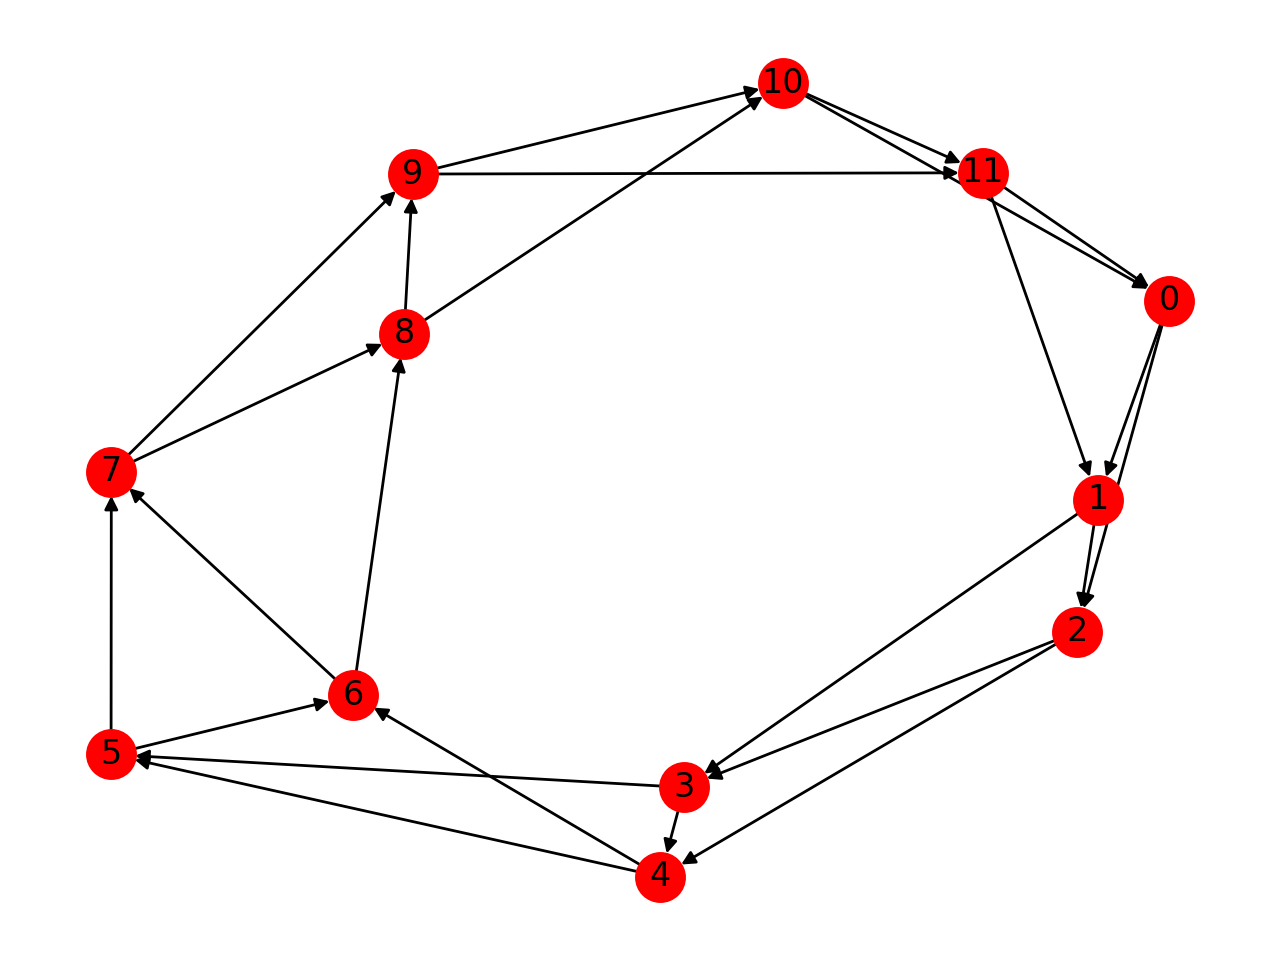
\includegraphics[scale=0.7]{figs/Graph_12_agents_k=2}
	\caption{Graph topology resulting from the \textit{-k 2} option.}
	\label{cycle_like_graph}
\end{figure}
\\
It can be seen that each agent \textit{i} has as out-neighbours the agents \textit{i+1} and \textit{i+2} and as in-neighbours the agents \textit{i-1} and \textit{i-2}. \\This can be formalized as follows:
\begin{equation}
	\text{N}^{\text{OUT}}_{i} = \left\{i+1, i+2, \dots , i+k  \right\}
\end{equation}
\begin{equation}
	\text{N}^{\text{IN}}_i = \left\{i-1, i-2, \dots, i-k  \right\}
\end{equation}
It's important to treat the numbers of the agents as if they were ordered with an agent following another one. This means that to the last agent $N$ follows the agent $0$.

\subsection{Loss function calculation}
The loss function (described in Eq. \ref{EQ1.7}) is implemented in the Python function called \textit{loss\_softmax}. It has three parameters:\\
\begin{itemize}
	\item \textit{all\_theta}: the matrix with the current estimation of $\theta^*$;
	\item \textit{category\_count}: the number of categories in the dataset. In the IRIS dataset, this number is $3$;
	\item \textit{personal\_dataset}: represents the dataset accessible to the considered agent.
\end{itemize}
The only addition to the function is the calculation of the \textit{const\_to\_subtract}, a constant used to prevent the overflow. The property used to justify the use of this method is the following:
\begin{equation}
	\dfrac{e^a}{e^b} = \dfrac{e^{a-c}}{e^{b-c}}
\end{equation}
where $c$ represent the constant to subtract and it is calculated as
\begin{equation}
	c = max \left\{ \theta^{1^\top}x, \dots,  \theta^{K^\top}x \right\}
\end{equation}

\begin{lstlisting}
def loss_softmax(all_theta, category_count, personal_dataset):
    the_sum = 0
    for index in range(0, len(personal_dataset)):
        denominator = 0
        const_to_subtract = find_const_to_subtract(all_theta, personal_dataset[index][0:4])
		
        for theta in all_theta:
            denominator = denominator + np.exp(np.dot(theta, personal_dataset[index][0:4]) - const_to_subtract)
		
        for category in range(0, category_count):
            if category == personal_dataset[index][4]:
                _exp = np.exp(np.dot(all_theta[category], personal_dataset[index][:4]) - const_to_subtract)
                _log = np.log(np.divide(_exp, denominator))
                the_sum = the_sum - _log
	
	return the_sum
\end{lstlisting}

This function could be omitted because it is not needed for solving the problem. It is used only for debug purpose as it is needed to draw the graphics of the overall loss function and to demonstrate that the cost gets minimized.

\subsection{Gradient calculation}
Given the nature of the method used to solve the problem, this is the most important piece of software. The gradient of the cost function has been calculated to be:
\begin{equation}
	\nabla_{\theta^{(k)}}J(\theta) = - \sum_{i=1}^{m} \left[ x^{(i)} \left( 1 \left\{ y^{(i)}=k \right\} -     \dfrac{exp\left(\theta^{(k)^{\top}}x^{(i)} \right)}{ \sum_{j=1}^{K} exp\left(\theta^{(j)^{\top}}x^{(i)} \right)}      \right) \right]
	\label{gradient_softmax}
\end{equation}

The Python function \textit{gradient\_softmax} calculate the value of the equation \ref{gradient_softmax}, using the same method saw in the previous section to prevent overflow.

\begin{lstlisting}
def gradient_softmax(all_theta, category_count, dimensions, personal_dataset, normalized):

    thetas = np.zeros(dimensions)

    if normalized:
        m = len(personal_dataset)
    else:
        m = 1

    for index in range(0, len(personal_dataset)):
        denominator = 0
        const_to_subtract = find_const_to_subtract(all_theta, personal_dataset[index][0:4])

        for theta in all_theta:
            denominator = denominator + np.exp(np.dot(theta, personal_dataset[index][:4]) - const_to_subtract)

        for category in range(0, category_count):
            coeff = 0
            if category == personal_dataset[index][4]:
                coeff = 1
            _exp = np.exp(np.dot(all_theta[category], personal_dataset[index][:4]) - const_to_subtract)
            coeff = coeff - np.divide(_exp, denominator)
            thetas[category] = thetas[category] - ((1 / m) * np.multiply(personal_dataset[index][:4], coeff))
    return thetas
\end{lstlisting}

\subsection {Reaching consensus}

In this section it will be explained how the consensus is reached.\\

The distributed sub-gradient method is an iterative algorithm, so it make use of a cycle in which the calculations are made. In the Python script there is a constant, called \textit{MAX\_ITERATIONS}, that represents the limit of iterations that can be made. \\
The first thing done in the cycle is the calculation of the step-size, basing the computation on the type chosen from the command line argument.

\begin{lstlisting}
    if alpha_type == "diminishing":
        alpha = psi_coefficient * (1 / tt) ** alpha_coefficient
    else:
        alpha = alpha_coefficient
\end{lstlisting}
If a diminishing step-size is chosen, then the formula implemented is
\begin{equation}
	\alpha_t = \psi \left( \dfrac{1}{t} \right)^\gamma
\end{equation}
otherwise, it is used a constant step-size defined as follows:
\begin{equation}
	\alpha_t = \gamma
\end{equation}
with $t$ indicating the current iteration. \\

After this, the state of each agent is updated using the current state and the states of the in-neighbours. The new calculated state is then sent to all the out-neighbours. This is done with the following piece of code:
\begin{lstlisting}
    # Update with my previous state
    u_i = np.multiply(XX[tt - 1], weight)

    # Send the state to neighbors
    for node in graph.successors(rank):
        world.send(XX[tt - 1], dest=node)

    # Update with state of all nodes before me
    for node in graph.predecessors(rank):
        u_i = u_i + world.recv(source=node) * weight
\end{lstlisting}

The variables used here are:
\begin{itemize}
	\item  \textit{u\_i}: represents the current estimate of the state of the agents;
	\item \textit{world}: a variable used for communicating between nodes. It is made available by the MPI environment. It makes possible to the nodes to communicate between them, using functions like \textit{send} or \textit{recv};
	\item \textit{graph}: a variable representing the communication graph. It is created using the functions in the \textit{networkx} library. It has two main functions that can be called: \textit{successors(node)} that returns a list with the out-neighbours of the agent \textit{node} and \textit{predecessors(node)} that returns the in-neighbours;
	\item \textit{rank}: represents the identifier of each agent. It is made available by the MPI environment and it is an integer number, that goes from $0$ to \textit{number of agents - 1}.
\end{itemize}

Later, the value of the gradient is calculated, using the function name passed as command line argument:
\begin{lstlisting}
    # Variable for storing the gradient value    
    gradient = 0

    if function_name == "softmax":
        gradient = func.gradient_softmax(XX[tt - 1], category_n, dimensions, personal_dataset, normalized)
	
    elif function_name == "quadratic":
        gradient = func.gradient_quadratic(XX[tt - 1], category_n, dimensions, personal_dataset, Q, r)
	
    elif function_name == "exponential":
        gradient = func.gradient_exponential(XX[tt - 1], category_n, dimensions, personal_dataset)
	
    # Multiply the gradient value by alpha
    grad = np.multiply(alpha, gradient)
\end{lstlisting}
In particular, a variable is firstly defined to store the value of the gradient that will be calculated. After computing it, the gradient is multiplied by the step-size and the result is stored into the \textit{grad} variable. \\

After this phase, the state is updated using the gradient descent step:
\begin{lstlisting}
    for i in range(0, dimensions[0]):
        u_i[i] = np.subtract(u_i[i], grad[i])

    # Store  my new state
    XX[tt] = u_i
\end{lstlisting}
Since the \textit{u\_i} and \textit{grad} variable are matrices, then each component of the gradient (multiplied by the step-size) is subtracted from the current estimate of the state. The result is then stored into an array called \textit{XX}, which keeps in memory all the states at each iteration. \\

Consequently, the loss value is calculated at each iteration using the same function used to calculate the gradient. The result is then stored into an array that keeps in memory all the losses at each iteration:
\begin{lstlisting}
    if function_name == "softmax":
        losses[tt] = func.loss_softmax(XX[tt], category_n, personal_dataset)

    elif function_name == "quadratic":
        losses[tt] = func.loss_quadratic(XX[tt], category_n, dimensions, personal_dataset, Q, r)

    elif function_name == "exponential":
        losses[tt] = func.loss_exponential(XX[tt - 1], category_n, dimensions, personal_dataset)
\end{lstlisting}

After this, the stop conditions are checked: \\
\begin{lstlisting}
    # Checking epsilon reached condition
    if np.linalg.norm(np.subtract(XX[tt], XX[tt - 1])) < epsilon:
        buff = True

    # Rank 0 get all epsilon and check if all reached it
    buffer = world.gather(buff, root=0)

    # If true it set epsilon reached
    if rank == 0:
        if False not in buffer:
            epsilon_reached = True

    # Send epsilon reached to all agents
    epsilon_reached = world.bcast(epsilon_reached, root=0)

    # Check if all agent have reached epsilon condition and then exit from loop
    if epsilon_reached:
        if rank == 0:
            print("Exiting at iteration ", tt, "/", MAX_ITERATIONS, "Condition on epsilon reached")
        break
\end{lstlisting}

This is done in different steps:
\begin{enumerate}
	\item The following condition is firstly checked:
	\begin{equation}
		\left\lVert \theta_{t+1} - \theta_{t} \right\rVert
		\leq \varepsilon
	\end{equation}
	If it is met, the variable \textit{buff} is set to \textit{true}. 
	\item The agent \textit{0} collects all the values of \textit{buff} of each agent in the \textit{buffer} variable.
	\item Agent \textit{0} check if all the conditions in the \textit{buffer} variable are set to \textit{true}. If they are, then the variable \textit{epsilon\_reached} is set to \textit{true}.
	\item This variable is sent to all the other agents using the \textit{bcast} function of \textit{world} that broadcasts the value of the variable to all the nodes in the graph.
	\item As last step, all the agents exit from the main cycle if all of them have met the stop condition. 
\end{enumerate}

The last things done in the main cycle are to print the iterations to the screen. This is done by the following piece of code:
\begin{lstlisting}
    if tt in range(0, MAX_ITERATIONS, 100):
        if rank == 0:
            print("Iteration ", tt, "/", MAX_ITERATIONS)
\end{lstlisting}



%%%%%%%%%%%%%%%%%%%%%%%%%%%%%%%%%%%%
%%%%%%%%% CAPITOLO 2 %%%%%%%%%%%%%%%%
%%%%%%%%%%%%%%%%%%%%%%%%%%%%%%%%%%%%
\chapter{Results of simulations} \label{Cap2}
	To verify the correctness of the software, a couple of simulations were run, divided into two parts:
\begin{itemize}
	\item Minimization of the Softmax function to prove the convergence to the optimal value
		\item Application of the minimization algorithm to find the best coefficients to do the best predictions on the test dataset
\end{itemize}

\section{Minimization of the Softmax function}
The simulation has been carried out using a random directed graph made up of 17 agents, as shown in figure \ref{graph_17_agents}. \\
\begin{figure}[hb]
	\centering
	{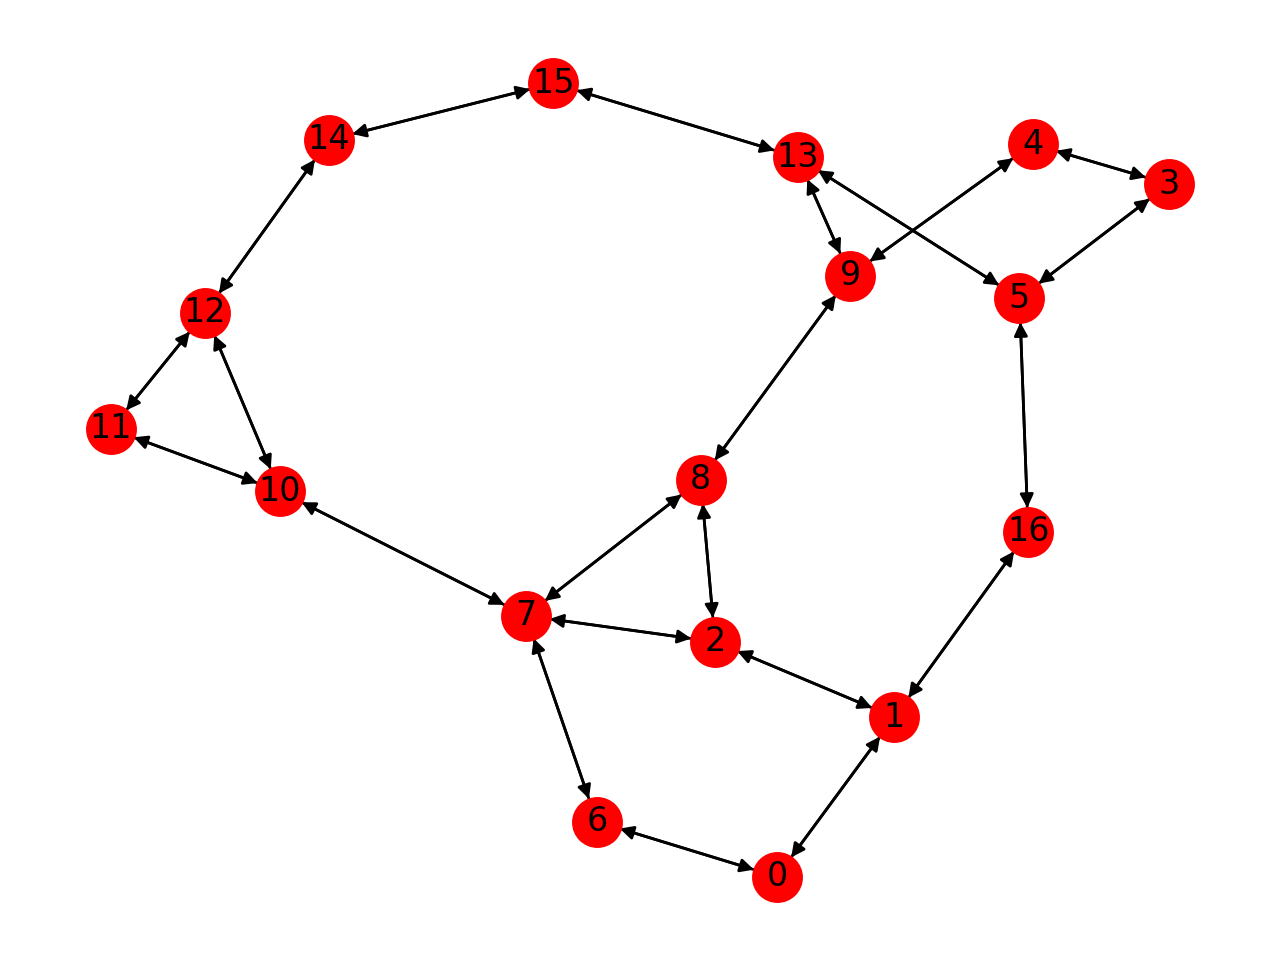
\includegraphics[scale=.55]{figs/Graph}}
	\caption{Communication graph used for the simulation.}
	\label{graph_17_agents}
\end{figure}

For completing this simulation, a diminishing step-size has been used, with the following formulation:
\begin{equation}
	\alpha_k = 0.01 \left( \dfrac{1}{k} \right) ^{0.4}
\end{equation}
with $k$ indicating the current iteration.\\
The problem to be solved is the one formulated in \ref{EQ1.7}. Let's suppose to indicate the whole dataset as $S$. Each agent $i$ can access to a limited set $s^i$ of examples contained in $S$. To each agent is given a set $s^i$, chosen as:
\begin{equation}
	\label{dataset_condition_union}
	S = \bigcup\limits_{i=1}^{17} s^i
\end{equation}
and 
\begin{equation}
\label{dataset_condition_intersection}
\bigcap\limits_{i=1}^{17} s^i = \emptyset
\end{equation}
In the simulation, the training set $S$ is composed by 120 examples, split into sets $s^i$ of 6 or 7 examples, chosen in order to equations \ref{dataset_condition_union} and \ref{dataset_condition_intersection} hold.  \\
The iterations run are 15000, sufficient enough to see the function approaching the convergence, but not sufficient enough to reach the minimum value of the function, calculated with \textit{MATLAB} to be $8.945$. The figure \ref{log_cost} shows in a logarithmic scale how the algorithm tends to minimize the cost value at each iteration. \\
\begin{figure}[hb]
	\centering
	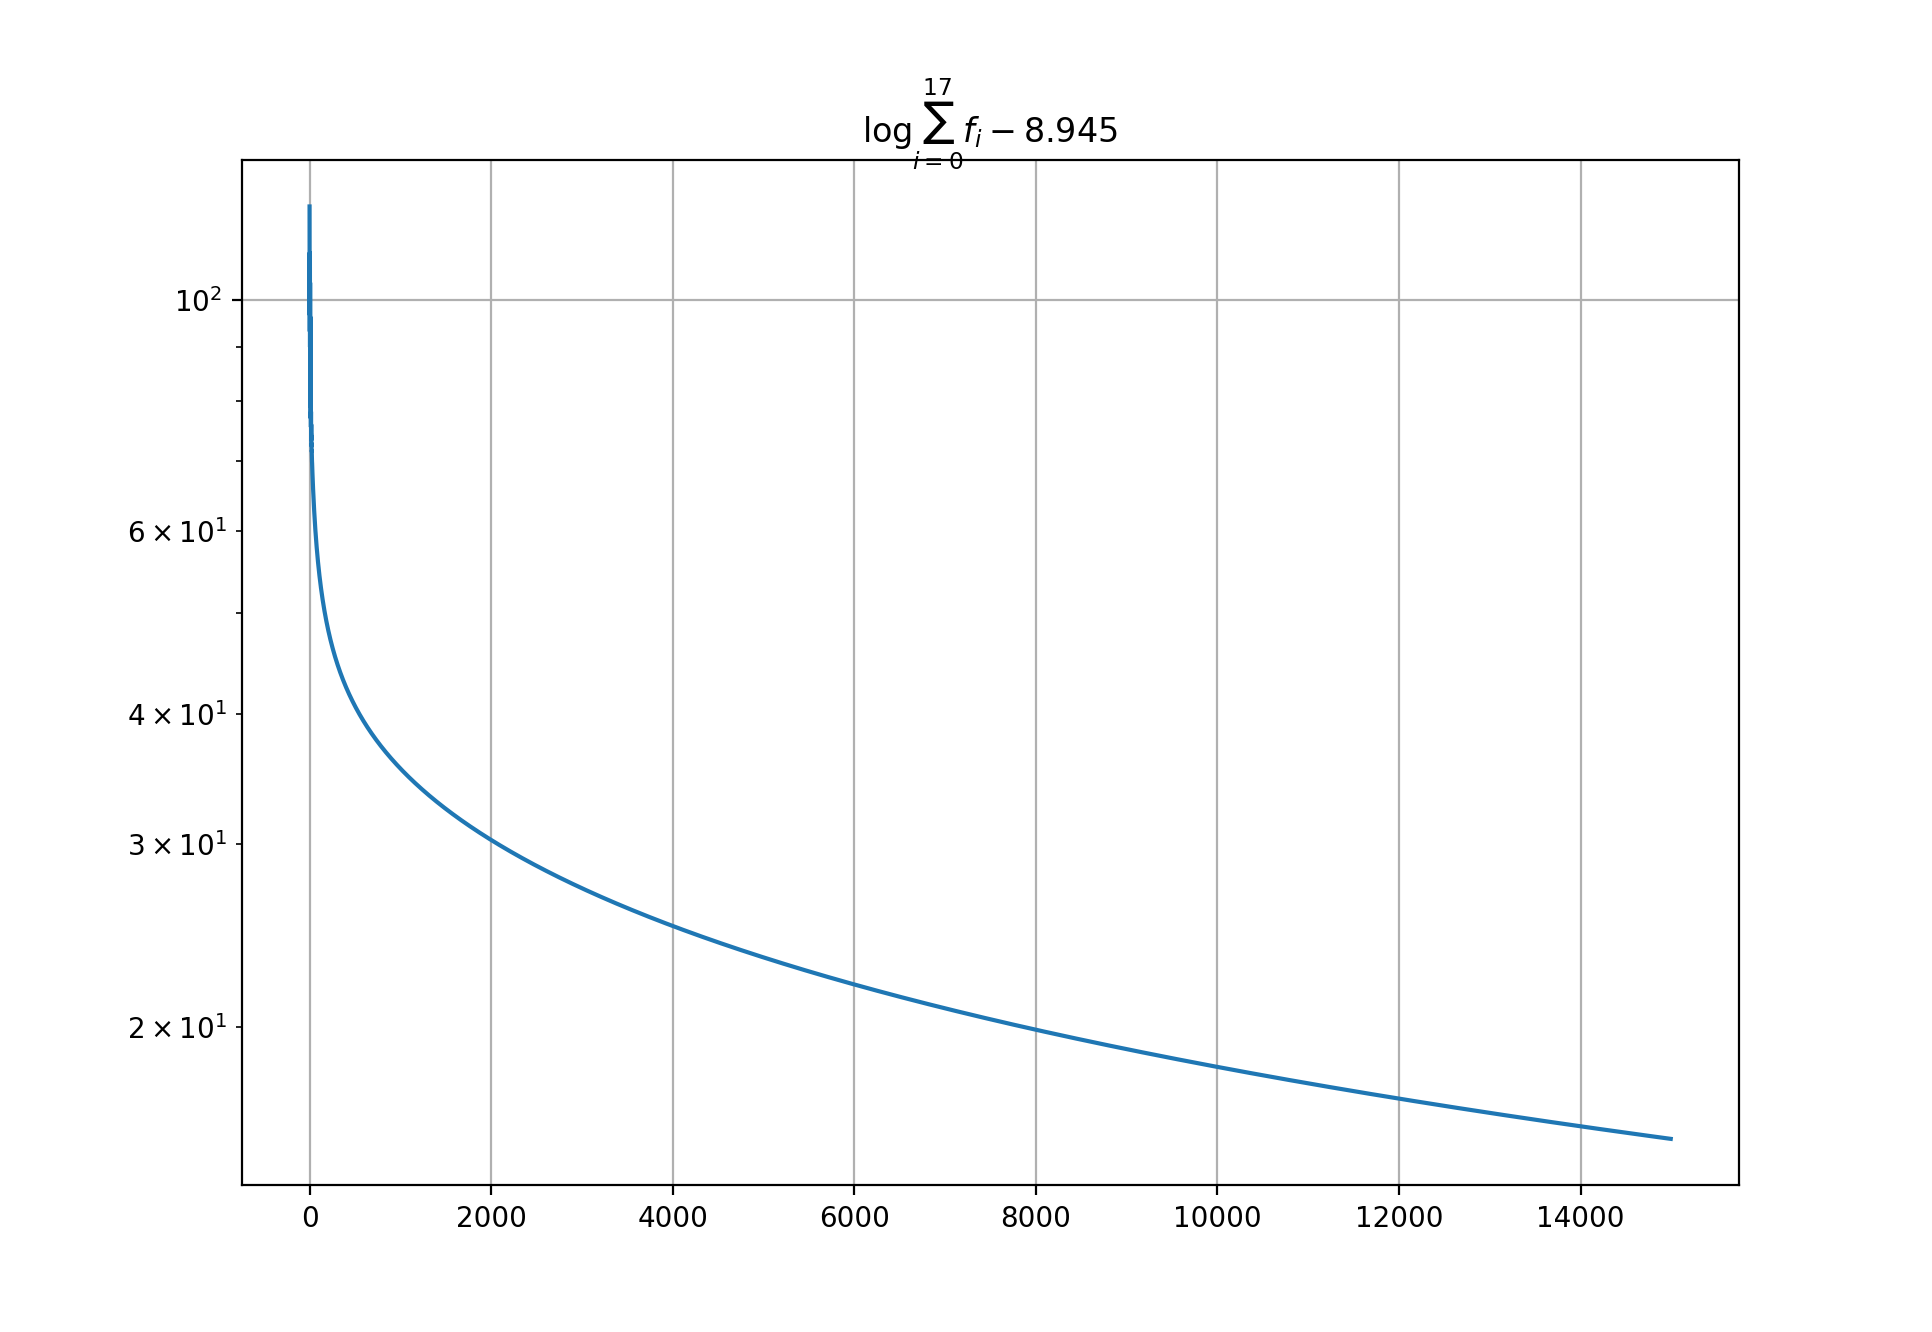
\includegraphics[scale=0.4]{figs/cost_log_scale}
	\caption{Value of the normalized cost function in a logarithmic scale over all the iterations. }
	\label{log_cost}
\end{figure}

The value of the cost function is shown in figure \ref{lin_cost} in a linear scale too, so it can be seen how the algorithm approaches the minimum value $\theta^{*}$ in order to have the minimum of the problem \ref{EQ1.7}.

\begin{figure}[ht]
	\centering
	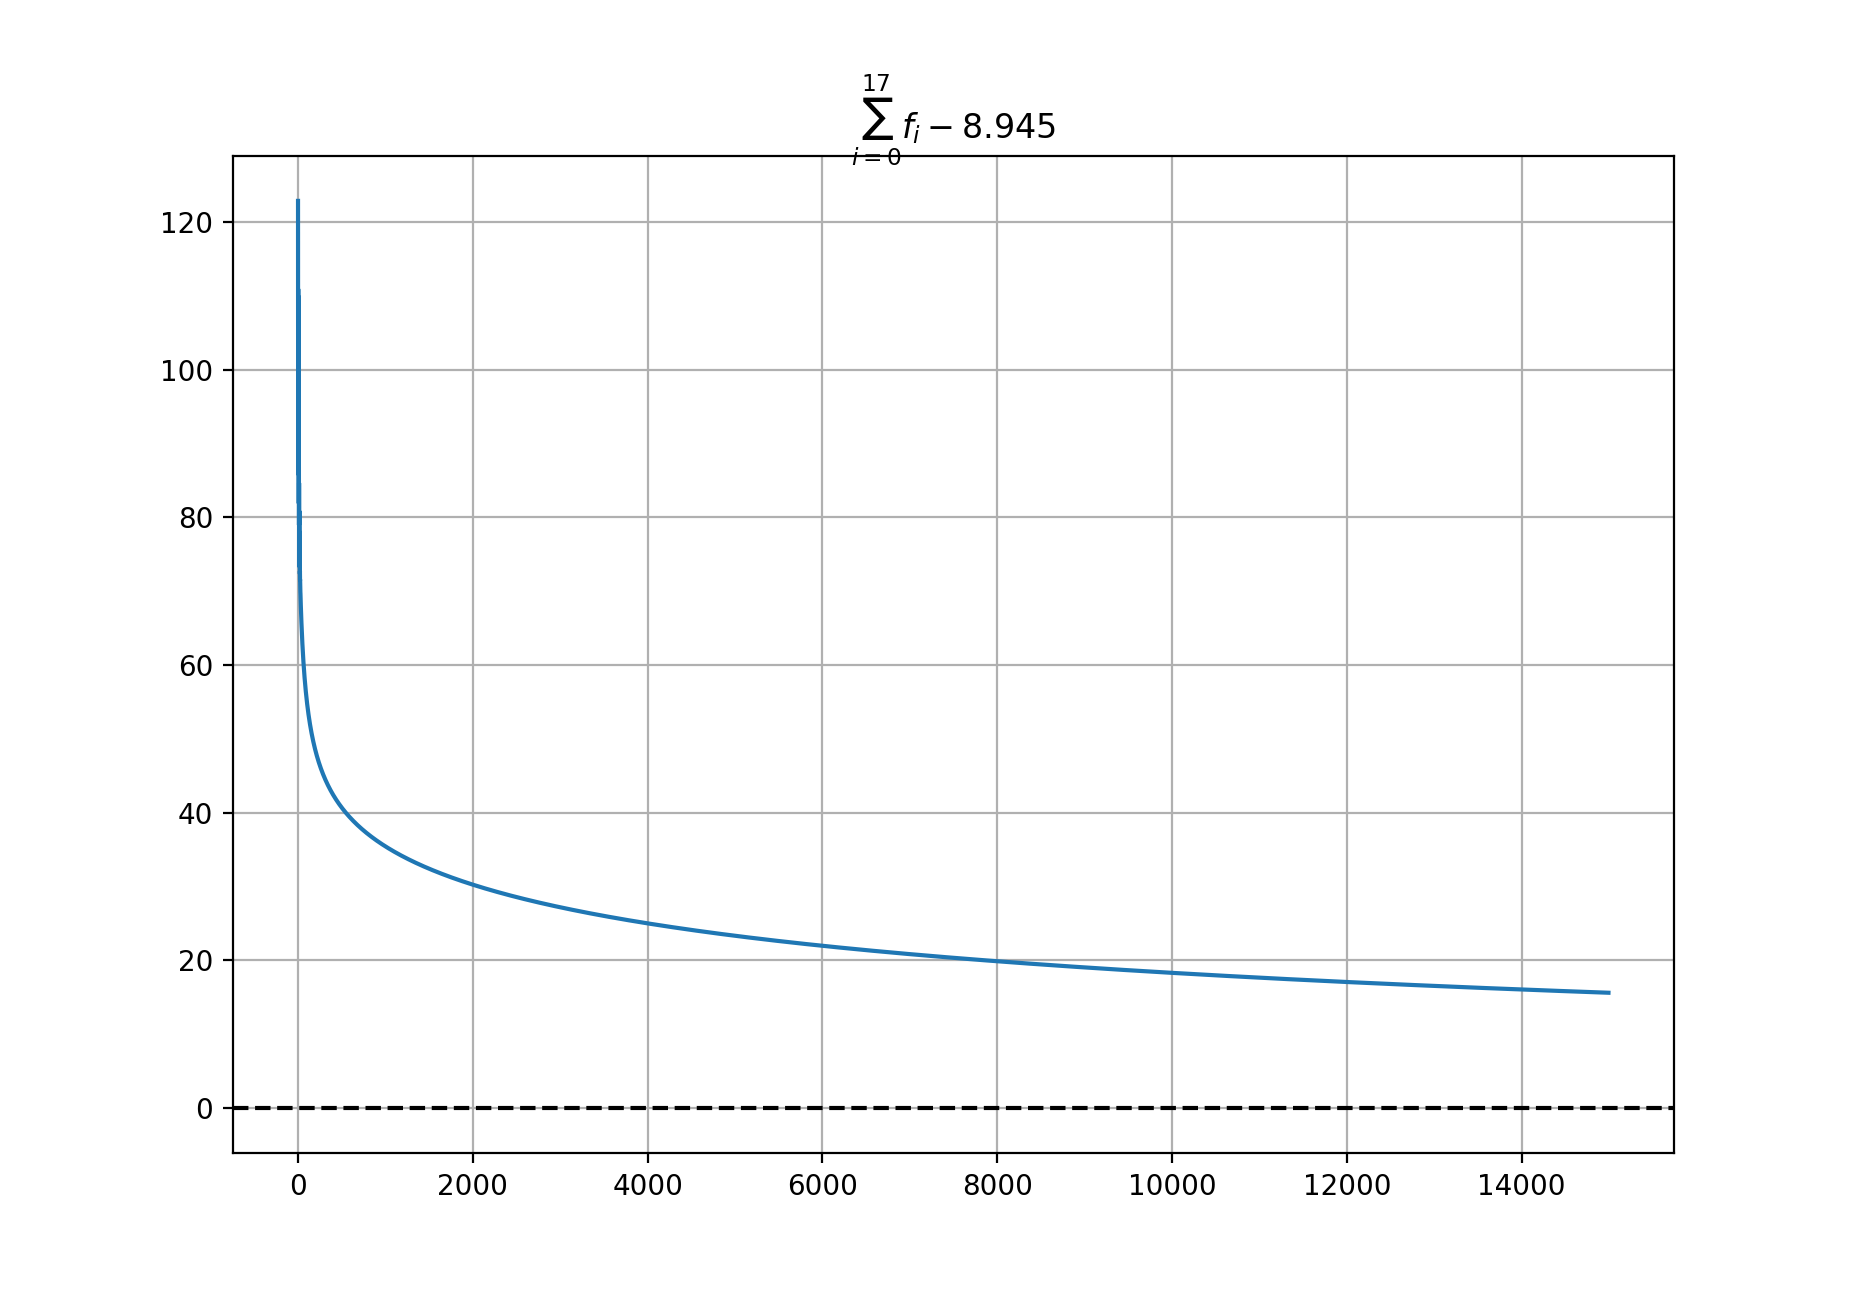
\includegraphics[scale=0.4]{figs/cost_linear_scale}
	\caption{Value of the normalized cost function in a linear scale. }
	\label{lin_cost}
\end{figure}

As can be seen in figure \ref{avg_consensus}, all the agents try to reach the consensus for each component of the local minimum of the problem. 

To better see the consensus, in this simulation the initial condition have been chosen to be random integer number between $-10$ and $+10$. With this choice is more visible the trend of the agents that try to reach consensus.

\begin{figure}[ht]
	\centering
	\begin{subfigure}{.5\textwidth}
		\centering
		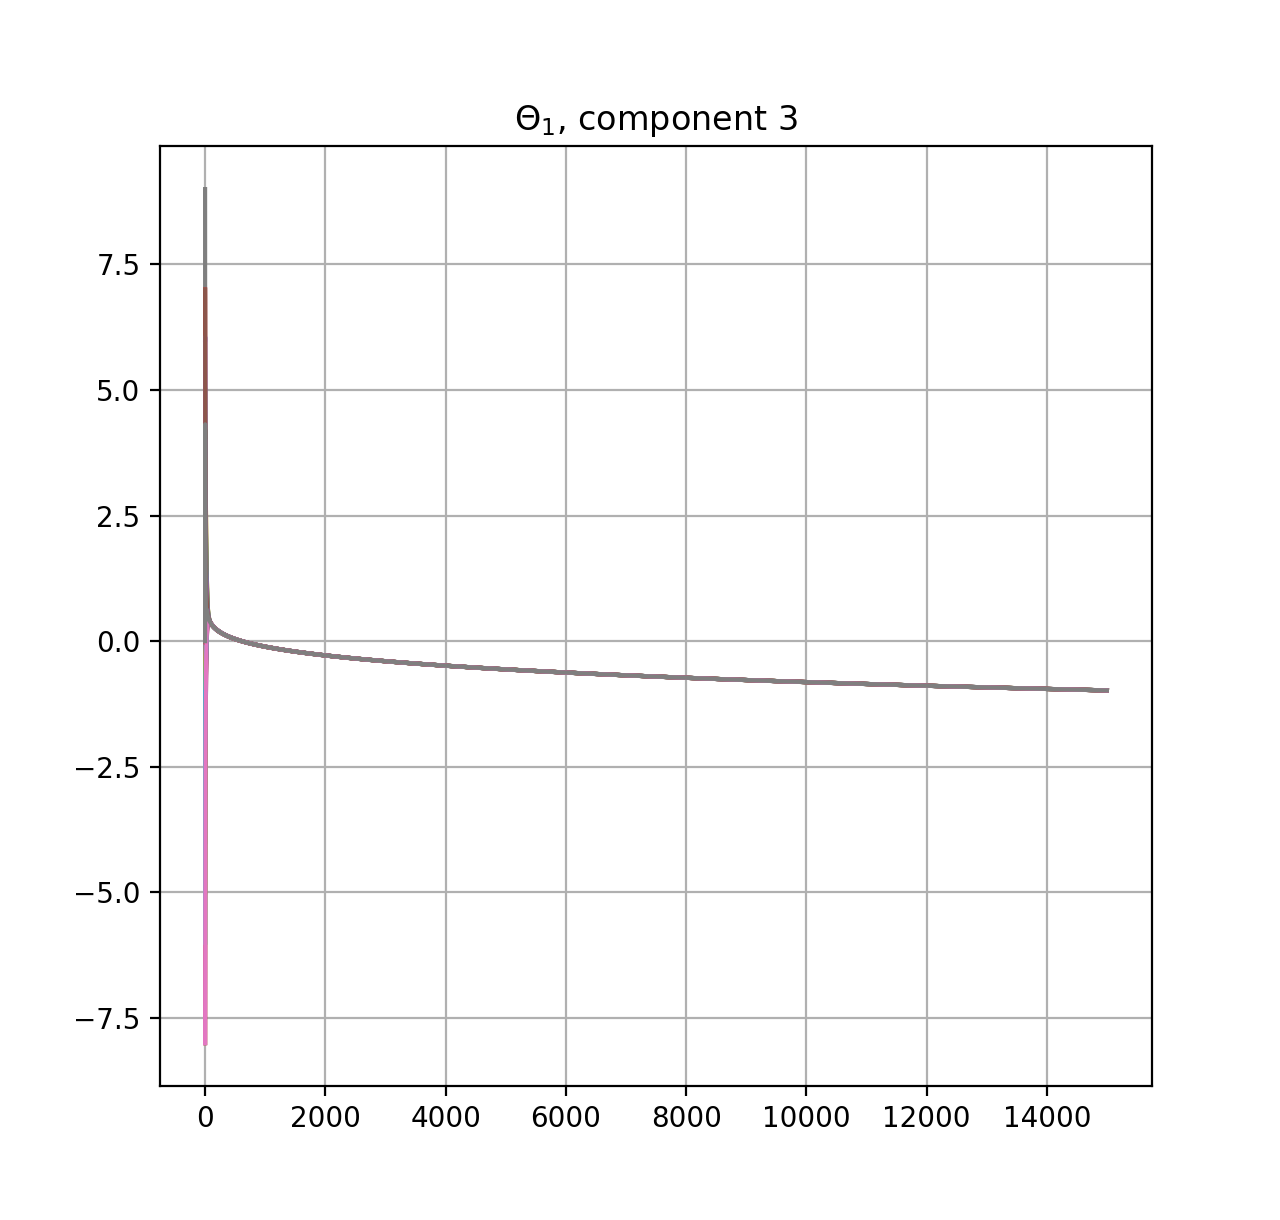
\includegraphics[scale=.4]{figs/theta_1_3_overall}
		\caption{Overall trend over all the iterations}
		\label{avg_consensus:overall}
	\end{subfigure}%
	\begin{subfigure}{.5\textwidth}
		\centering
		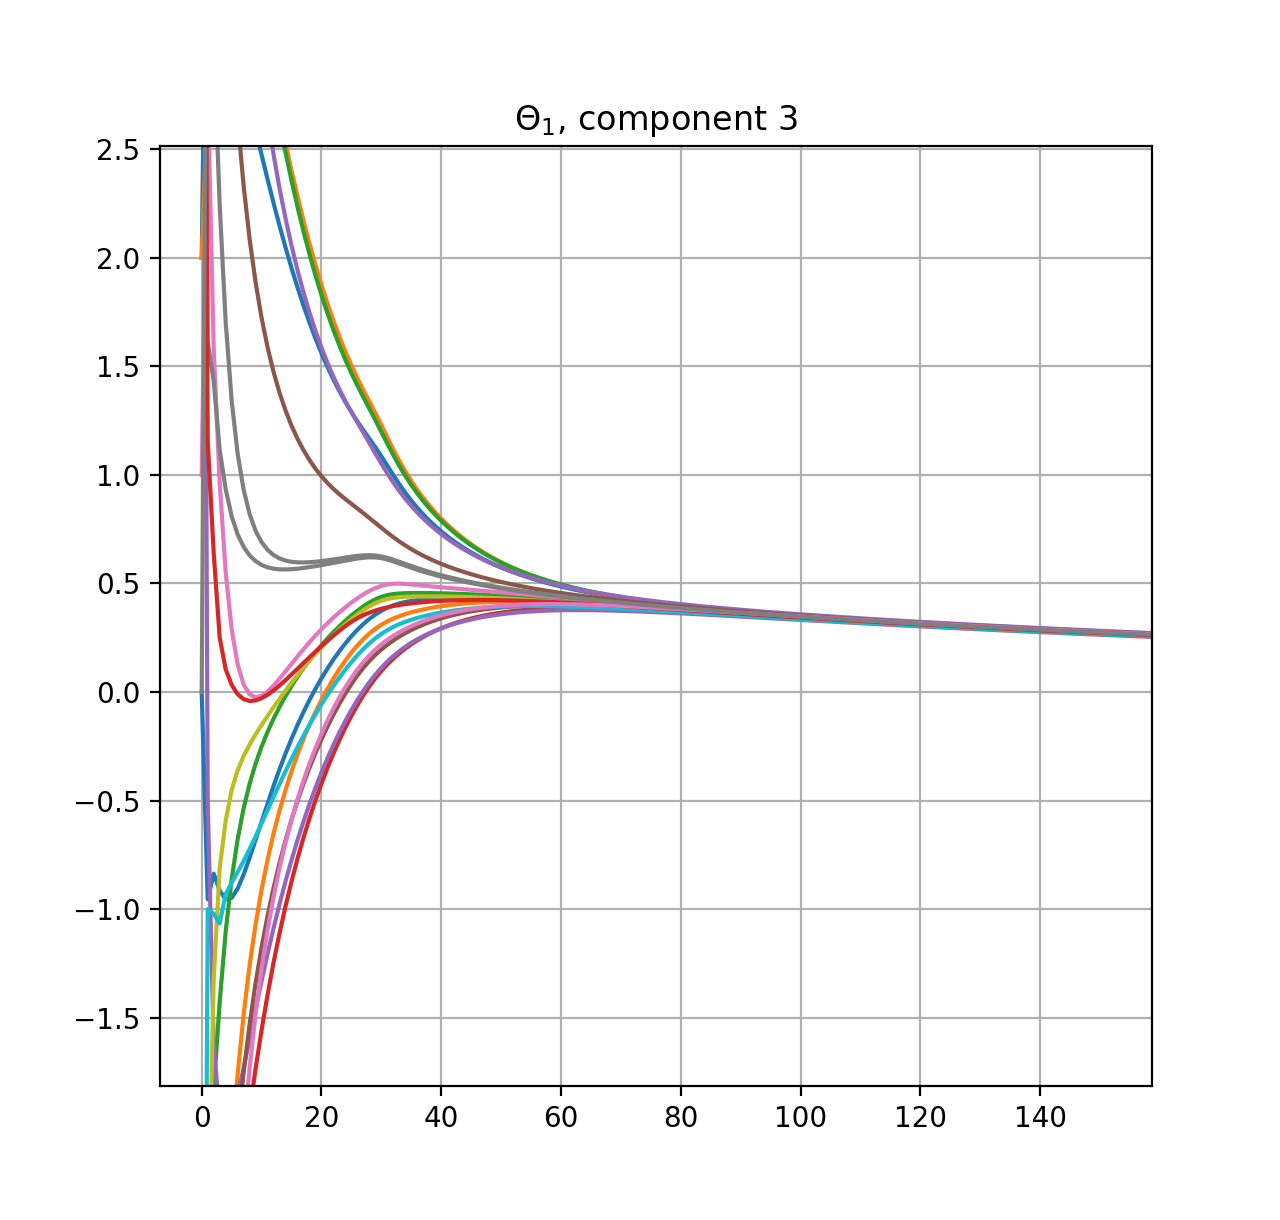
\includegraphics[scale=.4]{figs/theta_1_3_detail}
		\caption{Detail for the first 140 iterations}
		\label{avg_consensus:detail}
	\end{subfigure}
	\caption{Consensus on the third component of $\theta_1$}
	\label{avg_consensus}
\end{figure}

\section{Solving the Softmax Regression}
\subsection{Dataset, graph description and minimization function} \label{Sec2.1}
This dataset is composed of 150 instances, 120 of them used for training while the remaining 30 used for testing purpose. The instances contain 3 classes, each representing a type of Iris flower. Every instance has 4 features: sepal and petal length, sepal and petal width, expressed in $cm$. We tried different types of graphs, all of them chosen to be strongly connected. The results discussed in this chapter, if not differently noted, refer to cyclic graphs with a variable number of nodes. The program can minimize all kinds of loss functions. As shown in Chapter \ref{Sec1.2}, the quadratic and exponential functions can also be optimized, even if they don't guarantee useful results to apply to our problem. The minimization function used in this chapter is the one described in Chapter \ref{Subsec1.1.2}.

\subsection{Performance} \label{Sec2.2}
There are some key factors that influence \textit{the computational time}, \textit{the numbers of iterations necessary to reach consensus} and \textit{the accuracy of the results}. They are, but not limited to, the number of nodes, type of graph, step-size type and value, etc. \\

\subsection{Number of nodes} \label{Subsec2.2.1}
The Python program, thanks to the MPI platform, is capable of running on an arbitrary number of nodes. It was tested on as little as 2 nodes to as many as 60 nodes, which means that every node was processing the data of 2 instances (120 instances divided into 60 nodes). The best performances are obtained when the number of nodes corresponds to the number of physical cores of the machine where it runs. When the number of nodes exceeds greatly the number of physical cores, the resources are oversubscribed. In this case, the performances degrade notably as the nodes compete for cache and memory and the processors' schedulers are put in a difficult situation. On a 4-core test machine, a computation with 5000 iterations and 30 nodes is done in 5 minutes. The same machine can do the same number of iterations, but with 60 nodes, in 15 minutes. Therefore, to show the scalability of the software,  the following tests will be shown on a 4 nodes set-up and a 17 nodes setup (the same of Fig. \ref{graph_17_agents}) . \\

\subsection{Epsilon} \label{Subsec2.2.2}
This is a small constant used as stop condition. If the norm of the result of the current calculation differs less than $\varepsilon$ (chosen arbitrary small) from the previous, the algorithm is stopped. This is used as convergence stop condition. In fact, given the nature of the method used to minimize the cost function, the converge to the optimal value can be reached in a huge amount of time. To prevent this from happening, it has been used this condition.

\subsection{Learning rate} \label{Subsec2.2.3}
The step-size plays a big role in the speed of convergence of the algorithm. There are 3 kinds of step-size:
\begin{enumerate}
	\item fixed step-size: it has always the same value, which means $\alpha_{k+1} = \alpha_k$
	\item diminishing step-size: chosen such that 
	\begin{equation}
	\alpha_{k+1} < \alpha_k
	\end{equation}
	\begin{equation}
	\sum_{k=0}^{+\infty} \alpha_k = +\infty
	\end{equation}
	\begin{equation}
	\lim\limits_{k \to +\infty} \alpha_k = 0
	\end{equation}
	\item adaptive step-sizes: chosen with respect to Armijo or (limited) minimization rule.
\end{enumerate}
For reasons not discussed in this paper, it's not possible to use the last type of rules in a distributed problem, so the first two types have been used in these simulations.

\subsection{Initial condition} \label{Subsec2.2.4}
The agents start from an initial condition $x_0$, which represents a guess of the optimal value. The program was tested with random initial conditions for all agents and the consensus was still reached. To guarantee the repeatability of the experiments, the initial conditions in the tests are always set to a matrix full of ones.

\section{Four Nodes Setup} \label{Sec2.2}

\subsection{Fixed step-size} \label{Subsec2.2.4}
 We will first deal with a simple fixed step-size such as $\alpha^k = \alpha$, with $\epsilon = 10^{-3}$.\\ 
 A lot of step-size values have been tested, and the results of these test are shown in the following table.
\begin{scriptsize}
\begin{center}
\begin{tabular}{|>{\centering\arraybackslash}m{1.7cm}|>{\centering\arraybackslash}m{1.7cm}|>{\centering\arraybackslash}m{1.7cm}|>{\centering\arraybackslash}m{1.7cm}|}
\hline
\textbf{$\alpha$} & \textbf{Iteration required} & \textbf{Execution time in s} & \textbf{Wrong guesses}\\
\hline\hline
0.5 & overflow occurred & - & -\\
\hline
0.1 & \textgreater 10000 & \textgreater 15 & 2\\
\hline
0.05 & \textgreater 10000 & \textgreater 15 & 1\\
\hline
0.01 & 1968 & 2.8 & 1\\
\hline
0.005 & 1558 & 2.3 & 1\\
\hline
0.001 & 2114 & 3.1 & 0\\
\hline
0.0005 & 1619 & 2.3 & 2\\
\hline
0.0001 & 527 & 0.7 & 14\\
\hline
\end{tabular} \\
\end{center}
\end{scriptsize}

These results show a general truth about the step-size. If it is too little, the learning process proceeds in a very slow way and it requires a huge amount of iterations. If the learning rate is too high, the gradient descent will most probably overshoot the minimum and it will not converge.\\
Through trial and error, the step-size $0.001$ was chosen. It allows to reach good performances and the best accuracy: only 3.1 seconds are required to obtain 0 errors over the test dataset.

\subsection{Diminishing step-size} \label{Subsec2.2.5}
The diminishing step-size implemented is chosen to be:
\begin{equation}
\alpha_k = \psi \left( \frac{1}{k} \right)^{\gamma}
\end{equation}
Again, several tests were run by tweaking the multiplying constant and the exponent.\\ \\

\begin{scriptsize}
\begin{center}
\begin{tabular}{|>{\centering\arraybackslash}m{1.7cm}|>{\centering\arraybackslash}m{1.7cm}|>{\centering\arraybackslash}m{1.7cm}|>{\centering\arraybackslash}m{1.7cm}|>{\centering\arraybackslash}m{1.7cm}|}
\hline
\scriptsize{\textbf{$\psi$}} & \scriptsize{\textbf{$\gamma$}} & \scriptsize{\textbf{Iteration required}} & \scriptsize{\textbf{Execution time in s}} & \scriptsize{\textbf{Wrong guesses}}\\
\hline \hline
1 & 0.01 & overflow & - & -\\
\hline
1 & 0.1 & overflow & - & -\\
\hline
0.1 & 0.01 & \textgreater 10000 & \textgreater 15 & 1\\
\hline
0.1 & 0.5 & 349 & 0.5 & 0\\
\hline
0.1 & 0.1 & \textgreater 10000 & \textgreater 16 & 1\\
\hline
0.01 & 0.01 & 1852 & 2.7 & 1\\
\hline
0.01 & 0.1 & 1259 & 1.8 & 1\\
\hline
\end{tabular}\\
\end{center}
\end{scriptsize}

\noindent The best result is obtained in only 349 iterations, with $\psi = 0.1$ and $\gamma = 0.5$. This is done in roughly half of a second, obtaining no error and getting the result in a fraction of the time needed to obtain the same errors with a fixed step-size. A difference of 2 or 3 seconds may not seem important using the Iris Dataset, with a small dataset. In a set-up where a bigger dataset is involved, one may appreciate the advantages of this faster approach.



\section{Seventeen Nodes Setup} \label{Sec2.2}
The following results are the ones for the set-up shown in fig. \ref{graph_17_agents}. \\
The computation times are greatly larger than the ones shown earlier. This is because the tests involving 17 agents are carried out on a quad-core machine, which means that MPI oversubscribe the resources and the CPU scheduler are put at hard work. \\
The optimal step-size is different from the ideal step-size of the 4 nodes set-up. Only through several tests and experience is possible to find a good step-size to reduce the errors in the best way.



\begin{scriptsize}
\begin{center}
\begin{tabular}{|>{\centering\arraybackslash}m{1.7cm}|>{\centering\arraybackslash}m{1.7cm}|>{\centering\arraybackslash}m{1.7cm}|>{\centering\arraybackslash}m{1.7cm}|>{\centering\arraybackslash}m{1.7cm}|}
\hline
\scriptsize{\textbf{$\psi$}} & \scriptsize{\textbf{$\gamma$}} & \scriptsize{\textbf{Iteration required}} & \scriptsize{\textbf{Execution time in s}} & \scriptsize{\textbf{Wrong guesses}}\\
\hline \hline
0.1 &  0.1 & \textgreater 10000 & \textgreater 440 & 2\\
\hline
0.5 & 0.1 & \textgreater 1000 & \textgreater 440 & 2\\
\hline
0.9 & 0.1 & \textgreater 10000 & \textgreater 440 & 2\\
\hline
0.01 & 0.1 & 1894 & 83 & 2\\
\hline
0.1 & 0.5 & 698 & 30 & 2\\
\hline
0.5 & 0.5 & 1017 & 44 & 1\\
\hline
0.9 & 0.5 & 2409 & 107 & 0\\
\hline
0.01 & 0.5 & 318 & 13 & 14\\
\hline
0.1 & 0.01 & \textgreater 10000 & \textgreater 440 & 1\\
\hline
0.5 & 0.01 & \textgreater 10000 & \textgreater 440 & 2\\
\hline
0.9 & 0.01 & \textgreater 10000 & \textgreater 440 & 2\\
\hline
0.01 & 0.01 & 3717 & 164 & 2\\
\hline

\end{tabular}\\
\end{center}
\end{scriptsize}

The values in the table are shown in Fig. \ref{17_agents_performance} too. On the right axis are shown the iterations, in the left axis there are the numbers of error.

\begin{figure}[h]
	\centering
	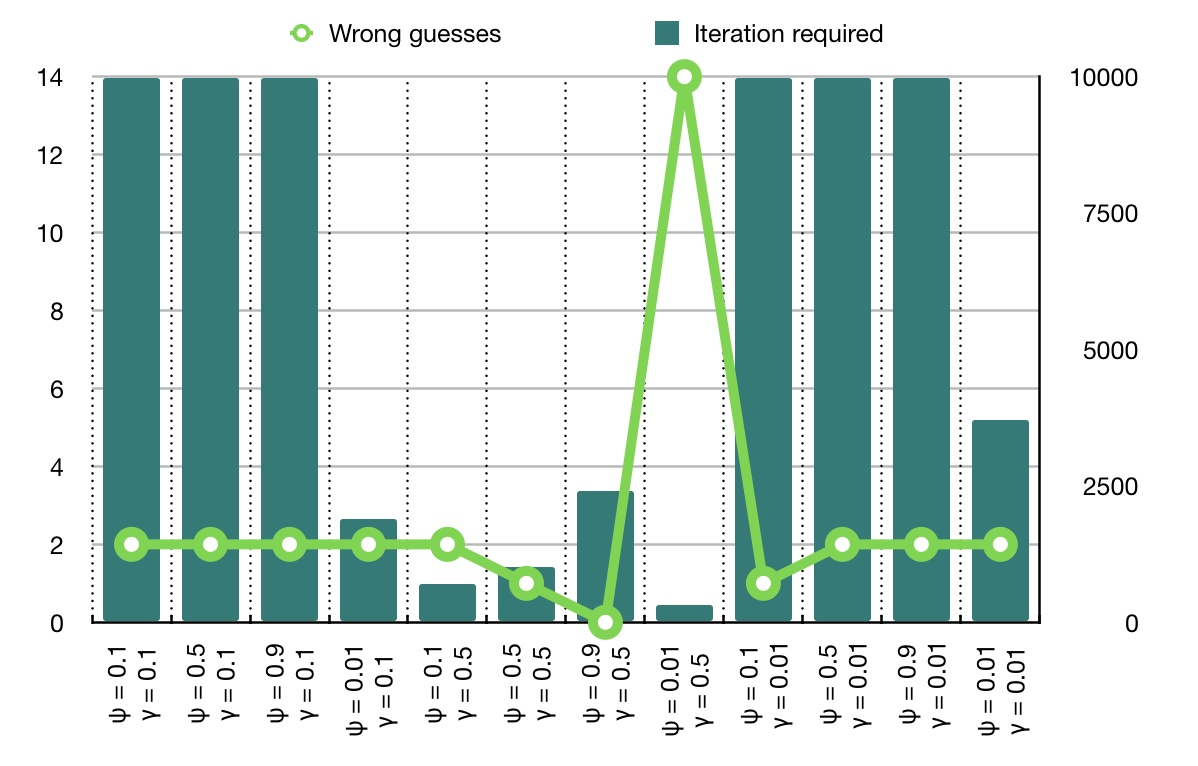
\includegraphics[scale=0.24]{figs/graphs_17_agents_performance}
	\caption{Results of the test for a graph with 17 agents.}
	\label{17_agents_performance}
\end{figure}

It can be seen that two optimal values of $\psi$ and $\gamma$ can be chosen.
Values of $\psi=0.5$, $\gamma=0.5$ gives only $1$ error in less than half of the iterations required to obtain $0$ errors with $\psi=0.9$ and $\gamma=0.5$. Basing on a given usage of the method, a user could prefer a couple of parameters instead of the other if he prefers velocity instead of accuracy.

%%%%%%%%%%%%%%%%%%%%%%%%%%%%%%%%%%%%%

%%%%% SVILUPPI FUTURI %%%%%%
\chapter*{Conclusions} % and future developments}
\addcontentsline{toc}{chapter}{Conclusions} %  and future developments}
In this work it has been resolved a \textit{Multinomial Logistic Regression} problem using \textit{MPI} in \textit{Python}. Each agent use a \textit{Distributed Sub-gradient Method} to update its own estimate of the optimal solution. At the end of the iterations, all the agents converge to the same solution.
%% Tutte le considerazioni finali sintetiche si fanno in base alla tabella dei risultati del capitolo 2.
%%%%%%%%%%%%%%%%%%%%%%%%%%

% %%%% APPENDIX %%%%%
% \appendix
% \chapter{Appendix title}
% %%%%%%%%%%%%%%%%%%%%

%%%%%%%%%% BIBLIOGRAPHY %%%%%%%%%%%%%%
\bibliography{bibliography}{}
\bibliographystyle{plain}   
\addcontentsline{toc}{chapter}{Bibliography}
%%%%%%%%%%%%%%%%%%%%%%%%%%%%%%%%%%%%%%

\end{document}
